%!TeX program=pdflatex
%!TeX encoding=utf8
%!TeX spellcheck = en_GB
%!TeX root = mailvortex_new.tex

\chapter{Introduction}
Almon Brown Strowger was owner of a funeral parlour in St. Petersburg. He filed a patent in Mach \nth{10} 1891 for an ``Automatic Telephone Exchange'' \cite{pulseDialingPatent}. This patent built the base for modern automated telephone systems. According to several sources he was annoyed by the fact that his local telephone operator was married to another undertaker. She diverted potential customers of Mr. Strowger to her huband instead causing him to lose business. In 1922 this telephone dialing system which is nowadays called pulse dialing became the standard dialing technology for more than 70 years until it was replaced by tone dialing. 

This dialing technology enabled automatic messaging for voice and text messages (e.g. telex) up until today and built the base technology for today's routed networks. 

These networks are building the base 

Numerous events in present and past have shown that data is broadly collected in the internet. Wether this is a problem or not may be a disputable fact. Undisputed is however that if data is not handled with care peoples are accused with numerous ``facts'' that are more than questionable. To show that this may happen even under complete democratic control we might refer to events such as the ``secret files scandal?? (or ``Fichenskandal'') in Switzerland. In the years  from 1900 to 1990 Swiss government collected 900'000 files in a secret archive (covering roughly 10\% of the natural and juristic entities within Switzerland at that time). 

A series of similar attempts to attack privacy on a global scale have been discovered by whistle blower Edward Snowden. The documents leaked in 2009 by him claim that there was a data collection starting in 2010. Since these documents are not publicly available it is hard to to prove claims based on these documents. However -- due to the fact that the documents were screened by a significant number of journalists spanning multiple countries, the information seems credible.

According to these documents (verified by \href{http://www.nrc.nl/nieuws/2013/11/23/nederland-sinds-1946-doelwit-van-nsa}{NRC}) NSA infiltrated more than 50k computers with malware to collect classified information. They furthermore infiltrated Telecom-Operators (executed by british GCHQ) such as Belgacom to collect data and targeted high member of governments even in associated states (such as the germans president mobile phone). A later published shortened list of ``selectors'' showed 68 telephone and fax numbers targeting enconomy, finance and agricultural parts of the german government.

This list of events shows that big players are collecting and storing vast amounts of data for analysis or possibly future use. The list of events shows also that the use of this data has in the past been at least partially questionable. As a part of possible counter measures this work analyses the possibility of using state of the art technology to minimize the information footprint of a person on the internet. 

We leave a vast information footprint in our daily communication. On a regular email we disclose everything in an ``postcard'' to any entity on its way. Even when encrypting a message perfectly with today's technology (S/MIME\cite{RFC2045} or PGP\cite{RFC2015}) leaves at least the originating and the receiving entity disclosed or we rely on the promises of a third party provider which offers a proprietary solution. Even in those cases we leak informations such as ``message subject'', ``frequency of exchanged messages'', ``size of messages'', or ``client beeing used''. A good anonymity protocol has therefore far more attributes to cover than the message itself. It includes beside the message all metadata and the traffic flows. Furthermore a protocol anonymising messages should not rely on the trust of infrastructure other than the infrastructure under control of the sending or receiving entity. 

Any central infrastructure is bound to be of special interest to anyone gathering data concerning the using entities of such a protocol. It furthermore may be manipulated in order to attack the messages or their flow. So central infrastructure has to be avoided.

In this work a new protocol is designed to allow message transfer through existing communication channels. These messages should be unobservable to any third party. This unobservability does not only cover the message itself but all metadata and flows associated with it. The protocol should be designed in such a way so that it is capable to use any type of transfer protocol. It should be even possible to switch protocols while have messages in transfer to allow media breaches (at least on a protocol level).

The new protocol should allow safe communication without the need of trusting the underlying transport media. Furthermore it is desirable that the usage of the protocol itself is possible without altering the immediate behaveour of the transport layer. That way it is possible to use the transport layers normal traffic to increase the noise in which information has to be searched. 

This work splits into multiple parts. In the first part we are collecting available researches and technologies. We emphasize in all technologies on the strength and weaknesses relevant to this work. In the second part we reassemble the parts to a new protocol. In the third part we analyse the protocol for fitness of the purpose. We try to find weaknesses and work out recommendations for the protocol usage. In the last part we discuss the results and try to summarize the findings. Try to elaborate to what extend the protocol fullfills the requirements of this work.

\chapter{Main Research Question}
The main topic of this thesis was defined as follows:
\begin{itemize}
	\item Is it possible to have specialized messaging protocol used in the internet based on ``state of the science'' technologies offering a high level of unlikability (sender and receiver anonymity) towards an adverser with a high budget and privileged access to internet infrastructure?
\end{itemize}

Based on this main question there are several sub questions grouped around various topics:

\begin{enumerate}
	\item What technologies and methods may be used to provide sender and receiver anonymity and unlinkability when sending messages against a potential adverser? (RQ1)
	\item How can entities utilizing these technologies and methods be attacked and what measures are  available to circumvent such attacks? (RQ2)
	\item How can attacks targeting anonymity of a sending or receiving entity be mitigated by design? (RQ3)
\end{enumerate}

\section{RQ1: Sending messages maintaining unlikability against an adverser}
This question covers the principal part of the work. As a result we get a list of suitable technologies. Based on this list we define a protocol combining these technologies and researches to a solution. This solution will be implemented and analysed for suitability based on the criteria defined.

\section{RQ2: Attacking unlinkability and circumvention}
Within this questions we look at common attacks and test resistance of the protocol based on the definition of the protocol.

\section{RQ3: Mitigation by design}
Within this question we define baselines in order to mitigate common attacks by design. We the flow these guidelines back into the protocol thus hardening it further.

% ********************************************************************************************************
% *** Methodes
% ********************************************************************************************************
\part{Methodes}
In this part of the thesis we collect requirements, definitions, methods, and existing research relevant to the topic of this thesis. We start with collecting requirements for the protocol. 

Having the requirements we collect numerous existing technologies on research and implementation level. Each of the technologies is quickly categorized and either further studied or rejected naming the reasons for rejection.

The list of technologies and research collected is big in this chapter. All relevant technologies either widely adopted or thoroughly researched should be included in this chapter. All Technologies and research are categorized. 

Technologies are always referenced through their respective standard. If applicable multiple standards may be part of the analysis. A very quick introduction into the protocol is given and then analysed for suitability for a specific problem addressed in this work.

Research are referenced by a paper. If applicable multiple related researches and papers are collected together into a bigger picture an then analysed for suitability concerning specific problem. If related to a standard technology links to that technology are provided where relevant.

\chapter{Requirements for an anonymising Protocol\label{sec:genRequirements}}
In the following sections we try to elaborate the main characteristics of the anonymising protocol. 

The main goal of the protocol is to enable Freedom of speech as defined in Article 19 of the International Covenant on Civil and Political Rights (ICCPR)\cite{iccpr}.
\begin{quote}
	everyone shall have the right to hold opinions without interference 
\end{quote}
and
\begin{quote}
	everyone shall have the right to freedom of expression; this right shall include freedom to seek, receive and impart information and ideas of all kinds, regardless of frontiers, either orally, in writing or in print, in the form of art, or through any other media of his choice.
\end{quote}

We imply that not all participants in the internet share this value. As of September \nth{1} 2016 Countries such as China (signatory), Cuba (signatory), Quatar, Saudi Arabia, Singapore, United Arab Emirates, or Myanmar did not ratify the ICCPR. Other countries such as United States or Russia did either put local laws in place superseding the ICCPR or made reservations rendering parts of it ineffective. We may therefore safely assume that freedom of speech is not given in the internet as a lot of countries explicitly supersede them.

We always have to keep in mind that we have no control over the flow of data packets in the internet. Packets may pass though any point of the world. It is not even possible to detect what way has a packet taken. The common network diagnostic tool \verb|tracert| respectively \verb|traceroute| tries to figure that out. But neither can a route of a packet beeing sent forseen nor can it be measured while or after sending. This is due to the fact that all routers along the way only decide for the next hop of a packet.

As an example of the problems analysing a packet route we may look at \verb|traceroute|. The mapage of traceroute of Linux tells us that \verb|traceroute| uses UDP, TCP, or ICMP packets with a short TTL and analyses the IP of the peer sending an TIME\_EXCEEDED (message of the ICMP protocol). This information is then collected and shown as a route. This route may be completely wrong. Some of the possible cases are described in the manpage.

The output of \verb|traceroute| is therefore not a reliable indication of route. Since routes do not have to be static and may be changed or even be alternating the output represents in the best case a snapshot of the current routing situation. We cannot be sure that data packets we are sending are passing only through countries accepting the ICCPR to the full extend.
\begin{figure}[H]
\begin{lstlisting}[language=bash,breaklines=true,prebreak={\mbox{\quad$\rhookswarrow$}},basicstyle=\footnotesize]
$ traceroute www.ietf.org
traceroute to www.ietf.org.cdn.cloudflare-dnssec.net (104.20.0.85), 64 hops max
1   147.86.8.253  0.418ms  0.593ms  0.421ms
2   10.19.0.253  1.177ms  0.829ms  0.782ms
3   10.19.0.253  0.620ms  0.427ms  0.402ms
4   193.73.125.35  1.121ms  0.828ms  0.905ms
5   193.73.125.81  2.991ms  2.450ms  2.414ms
6   193.73.125.81  2.264ms  1.961ms  1.959ms
7   192.43.192.196  6.472ms  199.543ms  201.152ms
8   130.59.37.105  3.465ms  3.138ms  3.121ms
9   130.59.36.34  3.904ms  3.897ms  4.989ms
10   130.59.38.110  3.625ms  3.333ms  3.379ms
11   130.59.36.93  7.518ms  7.232ms  7.246ms
12   130.59.38.82  7.155ms  17.166ms  7.034ms
13   80.249.211.140  22.749ms  22.415ms  22.467ms
14   104.20.0.85  22.398ms  22.222ms  22.146ms
\end{lstlisting}
\caption{A traceroute to the host www.ietf.org}
\end{figure}

\section{Anonymizing and unlinking}
If we are unable to limit the route of our packets through named jurisdictions we must protect ourselves from unintentionally breaking the law of a foreign country. Therefore we need to be anonymous when sending or receiving messages. Unfortunately most transport protocols (in fact almost all of them such as SMTP, SMS, XMPP or IP) use a globaly unique identifier for senders and receivers which are readable by any party which is capable of reading the packets. 

As a result anonymisation of a sender or a receiver is not simple. If messages are being sent through a relay at least the original sender might be concealed (Sender anonymity). By combining it with encryption we may even achieve a very simple form of sender and receiver pseudonymity. If cascading more relay like infrastructures and combining it with cryptography we might even achieve sender and receiver anonymity. This approach has however serveral downsides (see \ref{sec:remailer} and \ref{sec:mixnets} for details) and is easily attackable.

\section{Censorship Resistant}
In our scenario in \ref{sec:genRequirements} we defined the adverser as someone with superior access to the internet and its infrastructure. Such an adverser might attack a message flow in serveral ways:
\begin{itemize}
	\item Identify sender
	\item Identify recipient
	\item Read messages passed or extract meta information
	\item Disrupt communication fully or partially
\end{itemize}

We furthermore have to assume that all actions taken by a potential adverser are not subject to legal prosecution. This is due to the fact that an adverser trying to establish censorship may be part of a jurisdictions government. We may safely assume that there are legal exceptions in some jurisdiction for such entities.

In order to be able to withstand an adverser outlined above the protocol needs certain attributes. The message content needs to be unidentifiable by attributes or content. Whereas ``Attributes'' include meta information such as frequency, timing, message size, sender, protocol, ports, or recipient (list not conclusive).

\section{Controllable trust}
If we want to control trust we have to conclude that
\begin{enumerate}
	\item trust in an infrastructure is given due to the fact that it is under full control of either the sender or the recipient.
	\item trust in an infrastructure may not be necessary as the infrastructure is ideally unable to missuse data passed through it.
\end{enumerate}
In this thesis we work with both cases. We will however never trust a third party apart from sender and recipient (no even their providers of infrastructures).

\section{Reliable}
Any message sending protocol needs to be reliable in its functionality. If means of message transport are unreliable users tend to use different means for communication. 

\section{Diagnosable}
Reliability is somehow linked to transparent behaviour. This due to the fact that if something is generating a constant behaviour but we are unable to determine the reason for it (i.e. if we are expecting a different behaviour) we normally assume a malfunction. Therefore ``Reliable'' means not only stable by its behaviour. It means also diagnosable. User perception will not be ``Reliable'' if he is not able to determine causes for differences in observed and expected behaviour.

\section{Available}
Availability has two meanings in this context which do differ. A technology is available if\ldots
\begin{enumerate}
	\item a sender and a recipient have (or may have) the means of using it.
	\item the infrastructure is providing the service (as oposed to: ``is running in a degraded/faulty state unable to provide a service).
\end{enumerate}

The first meaning tells us that a protocol must run independently from infrastructure the user has commonly ready.

The second meaning tells us that messages must always be capable of flowing from the sender to the recipient. As infrastructure may fail at any time the protocol must offer the possibilities to send messages through alternate routes. This sounds easy and many protocols implement such redundancies already. However -- taking into account that sender and recipient is not known to a routing node this is a goal hard to achieve.

\section{Rough draft of Protocol Layers}
In order to fulfil the criteria given above we define a very rough idea of the protocol and its layers. The rough overview is given in figure \ref{fig:roughProtocolDesign}. The protocol should work on the base of onion routing. Unlike Tor (see \ref{sec:tor}) it should not rely on central infrastructures. it furthermore should not be limited to onionize messages. It should be capable of splitting and reassemble messages at any layer 

\begin{figure}[h]
	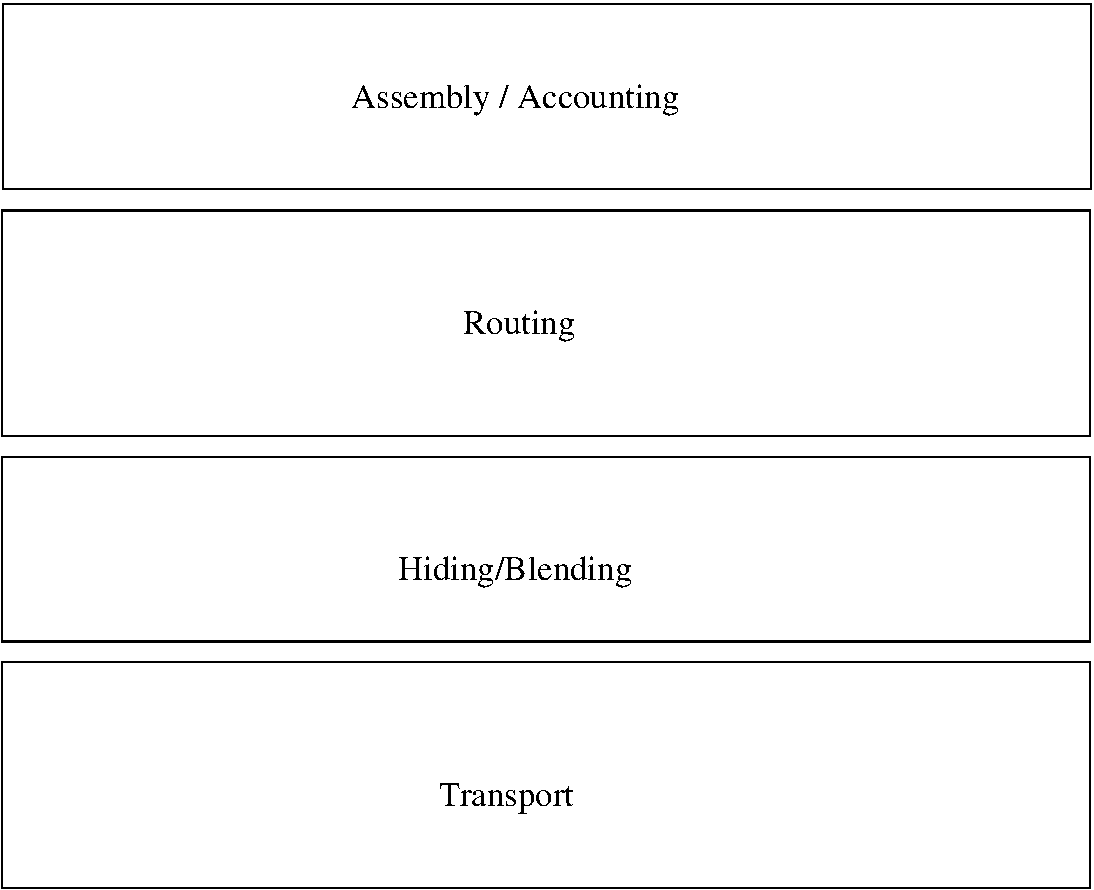
\includegraphics[width=\columnwidth]{inc/roughProtocolDesign}
	\caption{A first rough overview for the protocol}
	\label{fig:roughProtocolDesign}
\end{figure}	

The protocol itself should send messages through a well known transport protocol (``Transport'') which will be used for our messages. 

The messages will be hidden within regular messages already using that transport layer. In an ideal implementation messages sent by our protocol should be indistinguishable from regular messages (by computers and humans). In order to achieve this particular task we introduce a ``Hiding / Blending'' layer. This layer is normally specific to the underlying transport layer and may vary.

The ``Routing'' layer is the layer that receives and sends messages. It parses only the core protocol and the data processed here is completely independent from the underlying transport layer.

The ``Assembly / Accounting'' layer disassembles the received messages into its parts. It then recomposes and stores the messages for further routing. In order to avoid spaming over this media some kind of accounting will be involved.

\chapter{Existing Transport Layer Protocols}
In this chapter we have a look at various available transport layer protocol. The main goal is to identify strong candidates as a transport layer. Main focus lies on the following criterias:
\begin{itemize}
	\item Widely adopted (Ct1)\\
	      The more widely adopted and used a protocol is the harder it is for an adverser to monitor (due to the sheer mass), filter or block the protocol (censorship resistance).
	\item Reliable (Ct2)\\
	      Message transport between peers should be reliable. As messages may arrive anytime from everywhere we don not have means to synchronize the peer partners on a higher level without investing a considerable effort. In order to avoid this effort we do look for inherently reliable protocols.
	\item Symmetrical built (Ct3)\\
	      The transport layer should be built on a peer to peer base. All servers implement a generic routing which requires no prior knowledge of possible targets. This criteria neglects centralistic infrastructures.
\end{itemize}

\section{HTTP}
The HTTP protocol allows message transfer from and to a server and is specified in RFC2616 \cite{RFC2616}. It is not suitable as a communication protocol for messages due to the lack of notifications. There are some extensions which would allow such communications (such as WebDAV) but in general even those are not suitable as they require a continous connection to the server in order to get notifications. Having a ``rollup'' of notifications when connecting is not there by default but could be implemented on top of it. 

HTTP servers listen on standard ports 80 or 443 for incomming connects. The port 443 is equivalent to the port 80 except for the fact that it has a wrapping encryption layer (usually TLS). The incomming connects (requests) must offer a header part and may contain a body part which would be suitable for transferring messages to the server. The reply onto this request is transferred over the same TCP connection containing the same two sections.

HTTP0.9-HTTP/1.1 are clear text protocols which are human readable (except for the data part which might contain binary data). The HTTP/2 (as specified in \cite{RFC7540}) is using the same ports and default behaviour. Unlike HTTP/0.9-HTTP/1.1 it is not a clear text but a binary protocol. Headers and bodies of messages are sent as binaries. 

The protocol does definitely satisfy the first two main criteria (Ct1: Widely Adopted and Ct2: Reliable).

The main disadvantage in terms as message transport protocol is that this protocol is not symetrically. This means that a server is always just ``serving requests'' and not sending actively information to peers. This Request-Reply violates criteria (Ct1: Symmetrically built) and makes the protocol not a primary choice for  message transport. 

\section{MQTT}
MQTT is an ISO standard (ISO/IEC PRF 20922:2016) and was formerly called MQ Telemetry Transport. The current standard as the time of writing tis document was 3.1.1 \cite{mqtt}. 

The protocol runs by default on the two ports 1883 and 8883 and may be encrypted with TLS. MQTT is a publish/subscribe based message passing protocol which is mainly targeted to m2m communication. This Protocol requires the receiving party to be subscribed in a central infrastructure in order to be able to receive messages. This makes it very hard to be used in a system without centralistic infrastructure and having no static routes between senders and recipients.

The protocol does definitely satisfy the second criteria (Ct2: Reliable). It is in the area of enduser (i.e. Internet) not widely adopted thus violating Criteria 1 (Ct1: Widely Adopted). In terms of decentralistic design the protocol fails as well (Ct3: Symmetrically built).

\section{Advanced Message Queuing Protocol}
The Advanced Message Queuing Protocol (AMQP) was originally initiated by numerous exponents based mainly in finance related industries. The AMQP-Protocol is either used for communication between two message brokers, or between a message broker and a client\cite{amqp}.

It is designed to be interoperable, stable, reliable and safe. It supports either SASL or TLS secured communication. The usage of such a tunnel is controlled by the immediate sender of a message. In its current version 1.0 it does however not support a dynamic routing between brokers\cite{amqp}.

Due to the lack of a generic routing capability this protocol is therefore not suitable for message transport in a global generic environment.

The protocol satisfys partially the first criteria (Ct1: Widely Adopted), and fully satisfies the second criteria (Ct2: Reliable). However the third criteria is violated due to the lack of routing capabilities between message brokers (Ct3: Symmetrically built).

\section{Constrained Application Protocol (CoAP)}
The Constrained Application Protocol (CoAP) is a communication Protocol which is primarily destined to m2m communication. It is defined in RFC7252\cite{RFC7252}.  It is Defined as lightweight replacement for HTTP in IoT devices and is based on UDP.

The protocol does partially satisfy the first criteria (Ct1: Widely Adopted). The second criteria (Ct2: Reliable) is only partially fulfilled as it is based on UDP and does only add limited session control on its own.

The main disadvantage in terms as message transport protocol is that this protocol is not (like HTTP) symmetrically. This means that a server is always just ``serving requests'' and not sending actively information to peers. This Request-Reply violates criteria (Ct3: Symmetrically built) and makes the protocol not a primary choice for  message transport. 

\section{Web Application Messaging Protocol}
WAMP is a websockets based protocol destined to enable M2M communication. Like MQTT it is publish/subscribe oriented. Unlike MQTT it allows remote procedure calls (RPC).

The WAMP protocol is not widely adopted (Ct1: Widely Adopted) but it is definitely reliable on a per node base (Ct2: Reliable). Due to its RPC based capability unlike MQTT a routing like capability could be implemented. Symmetrical protocol behaviour is therefore not available but could be built in relatively easy.

\section{XMPP (jabber)}
XMPP (originally named Jabber) is a synchronous message protocol used in the internet. It is specified in the documents RFC6120\cite{RFC6120}, RFC6121\cite{RFC6120}, RFC3922\cite{RFC3922}, and RFC3923\cite{RFC3923}. The protocol is a very advanced chat protocol featuring numeros levels of security including end-to-end signing and object encryption\cite{RFC3923}. There is also a stream initiation extension for transferring files between endpoints \cite{xep0096}.

It has generic routing capabilities spanning between known and unknown servers.

The protocol itself seems to be a strong candidate as a transport layer as it is beeing used actively in the internet.

\fxfatal{figure out reliability of offline transfers and reliability in general}

\section{SMTP}
The SMTP protocol is currently specified in \cite{RFC5321}. It specifies a method to deliver reliably asynchronous mail objects thru a specific transport medium (most of the time the internet). The document splits a mail object into a mail envelope and its content. The envelope contains the routing information which is the sender (one) and the recipient (one or more) in 7-Bit ASCII. The envelope may additionally contain optional protocol extension material. \par

The content should be in 7-Bit-ASCII (8-Bit ASCII may be requested but this feature is not widely adopted). It is split into two parts. These parts are the header (which does contain meta information about the message such as subject, reply address or a comprehensive list of all recipients), and the body which contains the message itself. All lines of the content must be terminated with a CRLF and must not be longer than 998 characters excluding CRLF.\par

The header consists of a collection of header fields. Each of them is built by a header name, a colon and the data. Exact outline of the header is specified in \cite{RFC5322} and is separated with a blank line from the body. 

It \cite{RFC5321} furthermore introduces a simplistic model for mail communication. A more comprehensive model is introduced in the section \nameref{sec:mailTransport}. As the proposed model is not sufficient for a comprehensive end-to-end analysis.\par

Traditionally the message itself is mime encoded. The MIME messages are mainly specified in \cite{RFC2045}, and \cite{RFC2046}. MIME allows to send messages in multiple representations (alternates), and attach additional information (such as possibly inlined images or attached documents). 

SMTP is one of the most common messaging protocols in the internet (Ct1: Widely Adopted) and it would be devastating for business of a country if for censoring reasons this protocol would be cut off. The protocol is furthermore very reliable as it has built in support for redundancy and a throughout message design making it relatively easy to diagnose problems (Ct2: Reliable). All SMTP servers are normally capable of routing and and receiving messages. Messages going over serveral servers are common (Ct3: Symmetrically built) so the third criteria may be considered as fulfilled as well

SMTP is considered a strong candidate as transport layer.  

\section{SMS}
SMS capability was introduced in the SS7 protocol. This protocol allows the message transfer of messages not bigger than 144 character. Due to this restriction in size it is unlikely to be suitable for this type of communication as the keys beeing required are already sized similarly leaving no space for Messages or routing information.

Secondly the protocol is not widely adopted within the internet domain. There are gateways providing bridging functionalities to the SMS service. However -- the protocol itself is insignificant in the internet itself. 

\fxfatal{add credible source}

\section{MMS}
The Multimedia Messaging Service (MMS) is maintained by 3GPP (\nth{3} Generation Partnership Project). This protocol is manly a mobile protocl based on telephone networks.

\fxfatal{analyse criterias and add more information}

\section{Roundup for Transport Protocols}
\begin{table*}[t]
	\centering
	\begin{tabular}{|l|l|l|l|}\hline
		\diaghead{\theadfont protocol Criteria}{Protocol}{Criteria} & \thead{Ct1: Widely adopted} 	& \thead{Ct2: Reliable} & \thead{Ct3: Symmetrically built}\\\hline
		HTTP	 & $\checkmark$			& $\checkmark$		& $\times$\\              
		MQTT	 & \textasciitilde		& $\checkmark$		& $\times$\\              
		AMQP	 & \textasciitilde		& $\checkmark$		& $\times$\\
		CoAP	 & \textasciitilde		& \textasciitilde 	& $\times$\\
		WAMP	 & $\times$				& $\checkmark$		& \textasciitilde\\
		XMPP	 & $\checkmark$			& $\checkmark$		& $\checkmark$\\
		SMTP	 & $\checkmark$			& $\checkmark$		& $\checkmark$\\
		SMS\footnotemark[1] & 			& 					& \\
		MMS		 & $\checkmark$			& $\checkmark$		& $\times$\\\hline
	\end{tabular}	
	\caption{comparison of protocols in terms of the suitability criteria as transport layer}
	\label{tab:protoSuitCrit}
\end{table*}

In table \ref{tab:protoSuitCrit} we sum up all previously analysed protocols. We use ``$\checkmark$'' for a fulfilled criteria, ``\textasciitilde'' for a partially fulfilled criteria, and ``$\times$'' for a not fulfilled criteria. This overview shows in compact form which protocols have been identified as strong candidates for use as a transport layer in terms of an anonymising protocol. 

This table shows that strong identified candidates are SMTP (being already a message sending protocol on asynchronous base) and XMPP (a real time chat protocol able to attach files. This protocol features furthermore end-to-end encryption and signing). Both have the advantages that they are really wide adopted in the internet and do support additionally advanced content (such as alternatives or attachments).

\footnotetext[1]{omitted due to message size being too small}


\chapter{Existing Research and Implementations on the Topic}
\section{Anonymity}
\DeclareFixedFootnote{\omitted}{footnotes omitted in quote}
As Anonymity we take the definition as specified in \cite{anon_terminology}.
\begin{quote}
	Anonymity of a subject means that the subject is not identifiable within a set of subjects, the anonymity set.\omitted
\end{quote}
and
\begin{quote}
	Anonymity of a subject from an attacker's perspective means that the attacker cannot sufficiently identify the subject within a set of subjects, the anonymity set.\omitted
\end{quote}

Whereas the anonymity set is defined as the set of all possible subjects.

Especially the anonymity of a subject from an attacker's is very important to this paper. 

\subsection{$k$-Anonymity}
$k$-anonymity is a term introduced in \cite{k-anonymous:ccs2003}. This work claims that no one might be held responsible for an action if the action itself can only be identified as an action which has been taken by one unidentifiable entity out of $k$ entities.

The Document distinguishes between \textit{Sender $k$-anonymity} where the sending entity can only be narrowed down to a set of $k$ entities and \textit{Receiver $k$-anonymity} 

\fxfatal{say something about the size of $k$}

\fxfatal{add more content}

\subsection{$\ell$-Diversity}
In \cite{machanavajjhala2007diversity} an extended model of $k$-anonymity. According to the authors it is possible to break a $k$-anonymity set if there is additional Information available which may be merged into a data set so that a special entity can be filtered from the $k$-anonymity set. In other words if an anonymity set is to tightly specified a single additional background information might be sufficient to identify a specific entity in an anonymity set.

While it might be arguable that a $k$-anonymity in which a member is not implicitely $k$-anonymous still is sufficient for $k$-anonymity in its sense the point made in this work is definitely right and should be taken into account.

Their approach is to introduce an amount of invisible diversity into $k$-anonymous sets so that simple background knowledge is no longer sufficient to isolate a single member.

\subsection{$t$-Closeness}
While $\ell$-diversity protects the identity of an entity it does not prevent information gain. A subject which is in a class has the same attributes. This is where $t$-closeness\cite{li2007t} comes into play. $t$-closeness is defined as follows:

\begin{quote}
  An equivalence class is said to have $t$-closeness if the distance between the distribution of a sensitive attribute in this class and the distribution of the attribute in the whole table is no more than a threshold. A table is said to have $t$-closeness if all equivalence classes have $t$-closeness.
\end{quote}

\section{Zero Trust}
Zero trust is not a truly researched model in systems engineering. It is however widely adopted. 

We refer in this work to the zero trust model when denying the trust in any infrastructure not directly controlled by the sending or receiving entity. This distrust extends especially but not exclusively to the network transporting the message, the nodes storing and forwarding messages, the backup taken from any system except the client machines of the sending and receiving parties, and software, hardware, and operators of all systems not explicitly trusted.

As explicitely trusted in our model we do regard the user sending a message (and his immediate hardware used for sending the message), and the users receiving the messages. Trust in between the receiving parties (if more than one) of a message is not necessarily given.

\section{Pseudonymity}
As Pseudonymity we take the definition as specified in \cite{anon_terminology}.

\begin{quote}
	A pseudonym is an identifier of a subject other than one of the subject's real
	names. The subject which the pseudonym refers to is the holder of the pseudonym. A subject is pseudonymous if a pseudonym is used as identifier instead of one of its real names.\omitted
\end{quote}

\section{Undetectability}
As undetectability we take the definition as specified in \cite{anon_terminology}.

\begin{quote}
	Undetectability of an item of interest (IOI\index{Item of Interest}) from an attacker's perspective means that the
	attacker cannot sufficiently distinguish whether it exists or not.\omitted
\end{quote}

\section{Unobservability}
As unobservability we take the definition as specified in \cite{anon_terminology}.

\begin{quote}
	Unobservability of an item of interest (IOI) means
	\begin{itemize}
		\item undetectability of the IOI against all subjects uninvolved in it and
     	\item anonymity of the subject(s) involved in the IOI even against the other subject(s) involved in that IOI.
	\end{itemize}
	
\end{quote}

This part is very important. As we are heading for a censorship resistant solution unobservability is a key. As mentioned in this paper unobservability raises the bar of required attributes again ($\Rightarrow$ reads ``implies''):
\begin{eqnarray*}
	censorship\ resistance & \Rightarrow & unobservability\\
	unobserability         & \Rightarrow & undetectability\\
	unobserability         & \Rightarrow & anonymity
\end{eqnarray*}

So this means that we have to use an undetectable data channel in order to achieve censorship resistance.

\subsection{Ephemeral Identity}
In this work we use accounting on various levels. While we are dealing with anonymity accounting has still to be linked to some kind of identity for this reason we are introducing a term called ``ephemeral identity''.

\begin{quote}
	A Ephemeral identity is a temporary identity which is defined by the following attributes:
	\begin{itemize}
		\item It is an artificial identity
		\item It is only used for a short timespan
		\item It is not linkable to another identity
	\end{itemize}
\end{quote}

The key in this definition is the last point is crucial and at the same time hard to achieve.

\section{Single Use Reply Blocks and Multi Use Reply Blocks}
The use of single use reply blocks were first introduced by Chaum in \cite{chaum-mix}. The concept is that we have in our case a routing block which might be used up to $n$ times ($0<n<FIXME$)
\fxfatal{Add reference to Chaum}

\section{Censorship}
\subsection{Censorship Resistant}

\subsection{Parrot Circumvention}
\subsection{Censorship Circumvention}
\subsubsection{Covert Channel}
\subsubsection{Spread Spectrum}

\section{Cryptography}
\subsection{Symmetric Encryption}
\subsection{Asymmetric Encryption}
\subsubsection{RSA}
\fxfatal{Add content}\cite{Rivest:1978:MOD:359340.359342}

\subsubsection{Elliptic Curve Cryptogaphy}

\subsection{Homomorphic encryption}

\section{Routing}
\subsection{Mixing}
\fxfatal{suspectible to timing analysis}

\subsection{Onion Routing}
\fxfatal{suspectible to timing analysis ; mention example tarzan; mention example tor}

\subsection{Crowds}
\fxfatal{suspectible to timing analysis; mention example Freenet}

\subsection{Mimic routes}
\fxfatal{
	- mimics are chosen statically
	- garbage traffic is sent to mimics periodically
	- garbage traffic is replaced with real traffic when there’s real traffic
}

\subsection{Cryptopuzzles}
\fxfatal{Cryptopuzzles from "Theoretical and experimental methods for defending against DDOS attacks" by Mohammad Reza Khalifeh Solta}

\section{System Implementations}
The following sections describe 
\subsection{Concepts}
\subsubsection{DC Networks}
\subsubsection{MIX Networks\label{sec:mixnets}}
\subsubsection{Onion Routing}
\subsubsection{Remailer\label{sec:remailer}}

\subsection{Implementations}
The following sections emphasize on implementations of anonymising (and related) protocols regardless of their usage in the domain of messaging. It is a list of system classes or their specific implementations together with a short analysis of strength and weaknesses. Wherever possible we try to refer to original sources. This is however not always possible since some of these systems are no longer in use.
\subsubsection{Pseudonymous Remailer}
\subsubsection{Babel}
\subsubsection{Cypherpunk-Remailer}
\subsubsection{Mixmaster-Remailer}
\subsubsection{Mixminion-Remailer}
\subsubsection{Crowds}
\subsubsection{Tarzan}
\subsubsection{TOR \label{sec:tor}}
\subsubsection{Herbivore}
\subsubsection{Dissent}
\subsubsection{P5}
\subsubsection{Gnutella}
\subsubsection{Gnutella2}
\subsubsection{Freenet}
\subsubsection{Darknet}
\subsubsection{Sneakernet}
\subsubsection{Hordes}
\subsubsection{Salsa}
\subsubsection{Hydra-Onion}

\section{Known Attacks}
In the following sections we emphasize on possible attacks to an anonymity preserving protocols. In the following sections we describe classes of attacks. These attacks may be used to attack the anonymity of any entity involved in the message channel. In a later stage we test the protocol for immunity against these classes of attacks.

\subsection{Broken Encryption Algorithms}
\subsection{Attacks Targeting Anonymity}
\subsubsection{Hotspot Attacks}


\subsubsection{Message Tagging and Tracing}
\subsubsection{Side Channel Attacks}
\subsubsection{Timing Attacks}
\subsubsection{Sizing Attacks}

\subsubsection{Bugging Attacks}
\fxfatal{Bugging thru certificate/identity lookup}
\fxfatal{Bugging thru CRL lookup}
\fxfatal{Bugging thru DNS traffic}
\fxfatal{Bugging thru message content}

\subsection{Denial of Service Attacks}
\subsubsection{Censorship}
Where as traditional censorship is widely regarded as selective information filtering and alteration a very repressive censorship can even include denial of information flows in general. Any anonymity system not offering the possibility to hide in legitimate information flows is therefore not censorship resistant.
 
\subsubsection{Credibility Attack}
Another type of DoS attack is the credibility attack. While not necessarily a technical attack it is very effective. A system not having a sufficiently big user base is offering thus a bad level of anonymity due to the fact that the anonymity set is too small or the traffic concealing message flow is insufficient. 

In a credibility attack a systems reputation is degraded in such a way that the system is no longer used. This may be achieved in serveral ways. This is usually done by reducing the reputation of a system.

This may be achieved in several ways. Examples:
\begin{itemize}
	\item Disrupt functionality of a system.
	\item Publicly dispute the effectiveness of a system.
	\item Reduce the effectiveness of a system.
	\item Dispute the credibility of the system founders.
	\item Dispute the credibility of the infrastructure.
\end{itemize}

\chapter{Applied Methodes}
Based in the findings in this chapter we used the following methodology:
\begin{enumerate}
	\item Identify problem hotspots for a new protocol.
	\item Design a protocol which addresses the previously identified hotspots.
	\item Build a protocol prototype.
	\item Analyse the protocol for weaknesses using attack schemes.
	\begin{enumerate}
		\item Tagging/Bugging attacks
		\item Tracing attacks
	\end{enumerate}
\end{enumerate}

\section{Problem Hotspots}

\section{Protocol Design}
\begin{figure}[h]
	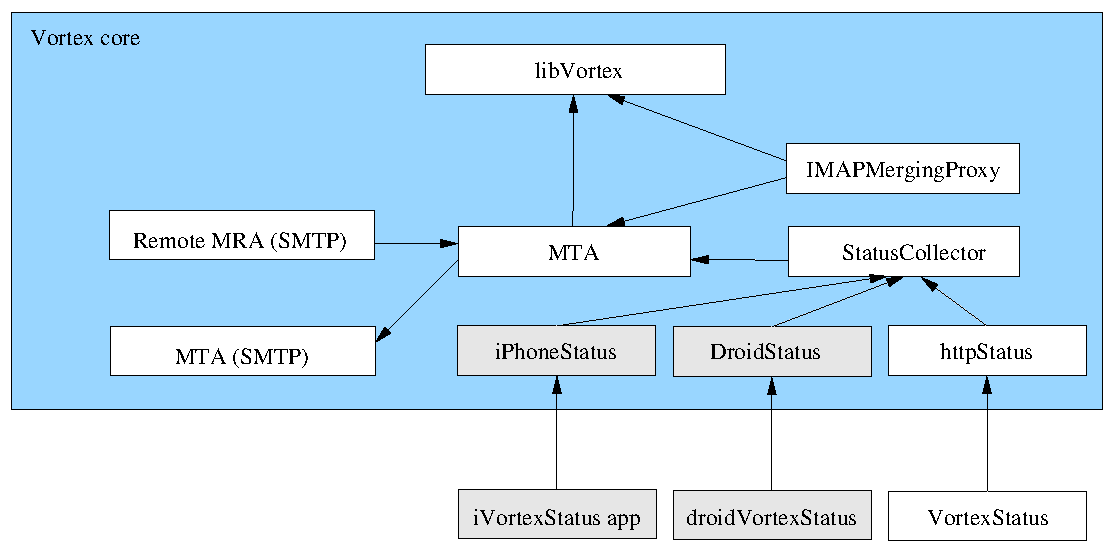
\includegraphics[width=\columnwidth]{inc/VortexModules}
	\caption{Overview of the Vortex modules}
	\label{fig:vortexModules}
\end{figure}

\section{Protocol implementation}

\section{Protocol Analysis}

\part{Results}
To verify the hypothesis made in this paper, and to analyse properties of the protocol in a real world scenario a library was implemented in Java which was capable of handling all message packets and the routing stack as a whole. The following paragraphs describe the protocol developed in general as a generic approach. Appendix \ref{app:asnone} gives the full ASN.1 representation of the protocol. 

It is important to notice that ASN.1 has no mean to express encrypted structures. Due to this fact we defined all encrypted fields as \verb|OCTET STRING|. The protocol offers according to the ASN.1 the possibility to store onionized information in an unencrypted form. This is meant for debuing purposes. At no point this should be used in a production environment.

The protocol described in the next chapter is independent from routing. At the moment capabilities include SMTP and XMPP. The protocol may be extended by adding new transport layer capabilities and their addressing schemes.

\chapter{MessageVortex - Transport Independent Messaging anonymous to \nth{3} Parties}
\section{Protocol Description}
\section{Accounting}
\section{Message Flows}
\section{Considerations for Building Messages}
\subsection{Timing of messages}
\subsection{Building Diagnostic Paths}
\subsubsection{Implicit Diagnostic}
\fxfatal{Add comments about messages splitting and returning to sender}

\subsubsection{Automatic Explicit Diagnostic}
\fxfatal{Add comments about error and diagnosis messages officially spliting of messages}

\subsubsection{On-Demand Explicit Diagnostic}
\fxfatal{Add comments about normal, error, and diagnosis messages beeing picked up by a routing block}

\section{Real World Considerations}
This approach is heavily dependent of the transport protocol and builds on top a new obfuscating/routing layer. For this system to become a real peer-to-peer approach some additional quirks are required. A message-Vortex-Account needs always an active routing handler. This routing handler may be introduced by new server capabilities or by having a device handling the routing from the client side. For this reason we built a RaspberryPi appliance capable of connecting to one (or more) accounts fetching incomming mails, analysing them and reroute them if necessary. Although the system is designed to be run on a RaspberryPi the software might be installed to any Java capable client. The RaspberryPi is just an affordable lightweight device which offers all required capabilities.

\chapter{Security Analysis}
\chapter{Additional Considerations}
\section{Storage of Messages and queues}
The storage of messages sent though MessageVortex should be handled with great care. It seems on the first sight a good idea to merge all messages in a globally available storage such as the mail account of the receiving entity. However -- In doing so we would discover the message content to the providing party of a mail account. Since we handled the message with great care and tremendous costs up until this point it would be careless doing so. 

Storing them in a localized and receiving entity controlled storage is definitely a good idea but leaves security considerations like a backup possibly to an end user. This might be better but in effect a questionable decision. There is however a third option. By leaving the message unhandled on the last entity of the MessageVortex chain we may safely backup the data without disclosing the message content. Merging the content then dynamically through a specialized proxy would allow the user tu have a unified view on his without compromising the security.

\fxfatal{implemented in prototype?}

\section{Economy of transfer}
\fxfatal{Write something about wasting bandwidth}

\part{Discussion}
\chapter{Anonymity}
\section{Effects of anonymous communication on behaveour}
\fxfatal{add content}\cite{postmes2001social}
